\section{Rates and optimality}
\label{sec:rates}

The error $\alpha^\star-\widehat\alpha$ is parametric on a grid of matching mesh when a function of the RKHS
separates the two contaminations, and no valid lower bound does better over such pairs (Section~\ref{sec:bothrates}). When they touch, a margin argument guarantees slower rates that depend on
the kernel, polynomial for Sobolev kernels and logarithmic for the Gaussian kernel (Sections~\ref{sec:linearmargin}
and~\ref{sec:touching}). The excess of the bound's own ramp recovers the parametric rate up to logarithmic factors on
the line with the Laplace kernel, for densities that cross once and under a condition on their likelihood ratio
(Theorem~\ref{thm:laplacerate}).

\subsection{A margin condition}
\label{sec:rate}

A rate needs a condition on the pair, and we use one, on how fast the regions separate below $\alpha^\star$.

\begin{assumption}[Polynomial margin]
\label{ass:margin}
There are constants $c_0>0$ and $\gamma\ge1$ such that $D_{\alpha^\star-\epsilon}(P,Q)\ge c_0\,\epsilon^\gamma$ for
all $\epsilon\in[0,\alpha^\star]$.
\end{assumption}

Validity and consistency hold for every pair, but by Section~\ref{sec:upper} no rate holds uniformly over all pairs,
and Assumption~\ref{ass:margin} restricts the pair only through its path. It suffices for $\epsilon\le\epsilon_0$, as the path is
nonincreasing, with $c_0(\epsilon_0/\alpha^\star)^\gamma$ in place of $c_0$. A margin of some form always exists when
$0<\alpha^\star<1$ (Lemma~\ref{lem:marginexists} of the supplement), Proposition~\ref{prop:newrates} of the supplement
gives the rate under any margin, and the assumption adds the polynomial speed. Exponents below $1$ are excluded, because
the rescaled path $(1-\alpha)D_\alpha(P,Q)$ is convex (Lemma~\ref{lem:pathconvex} of the supplement), so the path
leaves zero at most linearly, with a kink ($\gamma=1$) or tangentially ($\gamma>1$). The linear case holds when a function of the RKHS
separates the two contaminations (Section~\ref{sec:linearmargin}) and, for laws with continuous densities and a
continuous kernel, only if they are apart. In the following example the separating function takes three values.

\begin{example}[Separated contamination]
\label{ex:separated}
Let (A1) and (A2) of Assumption~\ref{ass:regularity} hold. Let $R$, $P_0$ and $Q_0$ be probability measures
concentrated on pairwise disjoint measurable sets $S_R$, $S_P$ and $S_Q$, let $\alpha^\star\in(0,1)$, and put
$P=(1-\alpha^\star)R+\alpha^\star P_0$ and $Q=(1-\alpha^\star)R+\alpha^\star Q_0$. Then $\TV(P,Q)=\alpha^\star$. If
moreover some $f\in\Hh$ takes the value $0$ on $S_R$, $1$ on $S_P$ and $-1$ on $S_Q$, then for every
$\alpha\in[0,\alpha^\star]$,
\[
D_\alpha(P,Q)\ \ge\ \frac{2(\alpha^\star-\alpha)}{(1-\alpha)\|f\|_\Hh}\ \ge\ \frac{2(\alpha^\star-\alpha)}{\|f\|_\Hh},
\]
so Assumption~\ref{ass:margin} holds with $\gamma=1$ and $c_0=2/\|f\|_\Hh$.
\end{example}

Such an $f$ exists for finite sets and a strictly positive definite kernel, as in
Section~\ref{sec:regions}, and for Mat\'ern kernels when the sets are bounded and apart (Section~\ref{sec:exproof} of
the supplement).

\subsection{Linear and slower margins}
\label{sec:linearmargin}

Whether the margin is linear depends on whether the contaminations touch. Write $P=P\wedge Q+\alpha^\star P_0$ and $Q=P\wedge Q+\alpha^\star Q_0$, where the contaminations $P_0$ and $Q_0$ are
the probability measures with densities $(p-q)_+/\alpha^\star$ and $(q-p)_+/\alpha^\star$.

\begin{proposition}[Touching contaminations]
\label{prop:newslope}
Let (A1) and (A2) of Assumption~\ref{ass:regularity} hold and let $0<\alpha^\star<1$, let $\mathcal X$ be a topological
space with its Borel sets, and let $\phi$ be continuous, as it is for a continuous kernel. Then
\[
\lim_{\epsilon\downarrow0}\frac{(1-\alpha^\star+\epsilon)\,D_{\alpha^\star-\epsilon}(P,Q)}{\epsilon}
\ \le\ \inf\big\{\|\phi(x)-\phi(y)\|_\Hh:\ x\in\supp P_0,\ y\in\supp Q_0\big\} .
\]
If the supports of $P_0$ and $Q_0$ meet, the limit is $0$ and Assumption~\ref{ass:margin} fails with $\gamma=1$. They
meet when $\mathcal X$ is a connected open subset of $\R^d$ and $P\neq Q$ have continuous Lebesgue densities $p,q$
such that $\{p=q\}$ has empty interior, as for any two distinct finite mixtures of nondegenerate Gaussian laws.
\end{proposition}

The limit exists by Lemma~\ref{lem:pathconvex}(ii) of the supplement. At the level $\alpha^\star-\epsilon$ one may keep
$P\wedge Q$ and add mass $\epsilon$ of $P_0$ near a point $x$ to the first law and of $Q_0$ near $y$ to the second,
whose embeddings then differ by about $\epsilon\{\phi(x)-\phi(y)\}$. With continuous densities and kernel, a linear
margin thus needs an open set on which $p=q$ that separates $\{p>q\}$ from $\{q>p\}$, and for a Mat\'ern kernel and
$P_0$ with compact support disjoint supports of $P_0$ and $Q_0$ also suffice (Proposition~\ref{prop:newgammaone} of the
supplement). Overlapping smooth laws, such as the overlap and shift designs of Section~\ref{sec:numerical}, fall
outside the linear case.

When the contaminations touch, the path leaves zero tangentially, at a speed set by how well the RKHS approximates
the indicator of $A=\{p>q\}$, with $p,q$ densities with respect to $P+Q$. For measurable $f$ with $0\le f\le1$ let
$\mathrm{err}(f)=\int|\mathbf 1_A-f|\,d|P-Q|$, where $|P-Q|$ is the total variation measure of $P-Q$, so that
$\mathrm{err}(f)=\alpha^\star-(\E_Pf-\E_Qf)$, and $\mathrm{err}(f)/2$ is the excess risk of the randomized classifier
that assigns $x$ to $P$ with probability $f(x)$, in the balanced problem whose Bayes classifier is $\mathbf 1_A$.

\begin{proposition}[Margin from an approximate witness]
\label{prop:newapprox}
Let (A1) and (A2) hold and let $0<\alpha^\star<1$. For every $f\in\Hh$ with $0\le f\le1$ and $f\neq0$, and every
$\epsilon\in[0,\alpha^\star]$,
\[
D_{\alpha^\star-\epsilon}(P,Q)\ \ge\ \frac{\epsilon-\mathrm{err}(f)}{(1-\alpha^\star+\epsilon)\,\|f\|_\Hh} .
\]
Hence $D_{\alpha^\star-\epsilon}(P,Q)\ge\epsilon/\{2\mathcal W(\epsilon/2)\}$, where
$\mathcal W(t)=\inf\{\|f\|_\Hh:\ f\in\Hh,\ 0\le f\le1,\ \mathrm{err}(f)\le t\}$.
\end{proposition}

In particular, if some $f\in\Hh$ with $0\le f\le1$ equals $1$ $P_0$-almost surely and $0$ $Q_0$-almost surely,
then $\mathrm{err}(f)=0$, and Assumption~\ref{ass:margin} holds with $\gamma=1$ and $c_0=1/\|f\|_\Hh$, since
$1-\alpha^\star+\epsilon\le1$. This is what we mean by a function of the RKHS separating the two contaminations;
Example~\ref{ex:separated} gives the constant $2/\|f\|_\Hh$ for an $f\in\Hh$ equal to $0$ on the common component, $1$
on one contamination and $-1$ on the other.

A trimming at level $\alpha$, before it is renormalized, is a part $P'\le P$ of mass $1-\alpha$, so it lowers the
integral of a $[0,1]$-valued function under $P$ by at most $\alpha$ and does not raise it under $Q$, and the
reproducing property turns the remaining gap into a lower bound on $(1-\alpha)D_\alpha$. The function $\mathcal W$ is
the approximation error behind the rates of kernel classifiers \citep{smale2003estimating,steinwart2008svm}: the closer
$\alpha$ is to $\alpha^\star$, the sharper $f$ must be across $\{p=q\}$, and the smoother the kernel, the more this
costs in $\Hh$. For a single transversal crossing on the line, Sobolev and Gaussian kernels make this quantitative.

\begin{proposition}[Sobolev kernels]
\label{prop:newsobolev}
Let $\mathcal X=\R$ and $k(x,y)=k_0(x-y)$, with $k_0$ continuous and integrable and
$c(1+\xi^2)^{-s}\le\widehat{k_0}(\xi)\le C(1+\xi^2)^{-s}$ for some $s>1/2$, as for the Laplace kernel, with
$s=1$, and the Mat\'ern kernel of smoothness $s-1/2$. Let $P,Q$ have densities $p,q$ that are continuous near a
point $x_0$, with $p\ge q$ almost everywhere on $(x_0,\infty)$ and $p\le q$ almost everywhere on $(-\infty,x_0)$, $p-q$
differentiable at $x_0$ with
$(p-q)'(x_0)>0$, $p(x_0)>0$, and $|P-Q|(\{x:|x-x_0|>t\})\le C'e^{-t/C'}$ for some $C'$ and all $t>0$. Then there are
$0<c_1\le c_2$ such that for all small $\epsilon>0$,
\[
c_1\,\epsilon^{(2s+3)/4}\ \le\ D_{\alpha^\star-\epsilon}(P,Q)\ \le\ c_2\,\epsilon^{(2s+3)/4} .
\]
\end{proposition}

Assumption~\ref{ass:margin} therefore holds with $\gamma=(2s+3)/4$ and with no smaller exponent, $\gamma=5/4$ for the
Laplace kernel. For the lower bound, an indicator smoothed at width $w$ has $\mathrm{err}(f)$ of order $w^2$, as
$|p-q|$ vanishes linearly at $x_0$, and $\|f\|_\Hh$ of order $w^{1/2-s}$, and $w\asymp\epsilon^{1/2}$ balances the two, while
the upper bound comes from explicit trimmings whose difference has vanishing moments near $x_0$. For $s>d/2$ the lower
bound extends to $\R^d$ when $|P-Q|$ has compact support and $\{p>q\}$ has a smooth compact boundary, with the exponent $1+(2s-1)/\{2(r+1)\}$ when
$p-q$ vanishes at least to order $r$ there (Theorem~\ref{thm:newsobolev} and Corollary~\ref{cor:newsobolev} of the
supplement), which is sharp on the line, at least for $s<3/2$, when it vanishes exactly to order $r$
(Proposition~\ref{prop:newupperone} of the supplement).

\begin{proposition}[Gaussian kernel]
\label{prop:newgauss}
Let $P,Q$ satisfy the hypotheses of Proposition~\ref{prop:newsobolev} on the laws, put $\ell_0=(p-q)'(x_0)$, the slope of $p-q$ at $x_0$, and let
$k(x,y)=\exp\{-(x-y)^2/(2\sigma^2)\}$ on $\R$. For every $c>\pi^2\sigma^2\ell_0/8$ and every $j\ge1$ there are
$\epsilon_0>0$ and $C_j<\infty$ such that, for $0<\epsilon\le\epsilon_0$,
\[
\exp(-c/\epsilon)\ \le\ D_{\alpha^\star-\epsilon}(P,Q)\ \le\ C_j\,\epsilon^j .
\]
\end{proposition}

With the Gaussian kernel the path is thus flatter at $\alpha^\star$ than every power, yet a margin of exponential type holds.
The approximant is an indicator smoothed by a band-limited density, which lies in the Gaussian RKHS
\citep{steinwart2006explicit} with a norm that grows like $\exp(c/\epsilon)$.

\subsection{The rate, and when it is optimal}
\label{sec:bothrates}
\label{sec:optimality}

Under the margin the error of the bound is at most of order $(n\wedge m)^{-1/(2\gamma)}$, up to the mesh of its
grid.

\begin{theorem}[Rate of the split-sample lower bound]
\label{thm:loratemain}
Let Assumptions~\ref{ass:regularity} and~\ref{ass:margin} hold, let $\alpha^\star<1$, and compute
$\widehat\alpha$ at level $\delta$ as in Proposition~\ref{prop:loconsistency}, with the batches of
Section~\ref{sec:betting}, $\lambda_{\max}=\tfrac12$ and the fractions \eqref{eq:fractions} of the supplement with initial
variance $v_0^2\le4$, on a grid of $J$ levels
fixed in advance whose mesh below $\alpha^\star$ is $\Delta_{\mathcal G}$. If $n\wedge m\ge10$, then for every $\eta\in(0,1)$, with
probability at least $1-\delta-\eta$,
\[
\alpha^\star-\Delta_{\mathcal G}-O\bigg(\bigg(\frac{\kappa}{c_0(1-\alpha^\star)v^2_{\min}}
\sqrt{\frac{1+\log(1/\delta)+\log(J/\eta)}{n\wedge m}}\bigg)^{1/\gamma}\bigg)
\ \le\ \widehat\alpha\ \le\ \alpha^\star ,
\]
with an absolute constant in the $O$.
\end{theorem}

This is parts (ii) and (iii) of Theorem~\ref{thm:lorate} of the supplement, which gives the constants. Below
$\alpha^\star$, on an event of high probability, the excess $\E_P\rp-\E_Q\rp-\alpha$ of the fitted ramps stays above a
multiple of $c_0(\alpha^\star-\alpha)^\gamma$ as soon as this exceeds a multiple of $(n\wedge m)^{-1/2}$, and betting
then rejects. Equating the two gives the rate, and the split adds the mesh and the factor $1/v^2_{\min}$. Part (i) of
that theorem removes $\log J$ when consecutive levels are far apart compared with the rate, as on the grid of
Corollary~\ref{cor:minimax} below. The constants are far from sharp.

When the regions separate linearly, no lower confidence bound improves the rate $(n\wedge m)^{-1/2}$, by the two-point
method of \citet{lecam1973convergence}: pairs whose total variations differ by $h$ of order $n^{-1/2}$ cannot be told
apart, and a bound valid at the pair with the smaller value must often fall short at the other.

\begin{proposition}[Two-point lower bound]
\label{prop:lower2pt}
Let $R$, $P_0$ and $Q_0$ be probability measures on $\mathcal X$ concentrated on pairwise disjoint measurable sets.
For $a\in(0,1)$ and $h\in[0,1-a)$ put $P_a=(1-a)R+aP_0$, $Q_a=(1-a)R+aQ_0$ and
\[
P_{a,h}=(1-a-h)R+(a+h)P_0,\qquad Q_{a,h}=(1-a-h)R+(a+h)Q_0 .
\]
Then $\TV(P_a,Q_a)=a$ and $\TV(P_{a,h},Q_a)=\TV(P_a,Q_{a,h})=a+h$. Let $\tilde\alpha$ be any measurable function of
the two samples and of an independent randomization such that $\Pp_{P_a,Q_a}(\tilde\alpha>a)\le\delta$. Then for every
$h\in(0,1-a)$,
\begin{align*}
\Pp_{P_{a,h},Q_a}\big(\TV(P_{a,h},Q_a)-\tilde\alpha\ge h\big)&\ge1-\delta-h\sqrt{n/\{2a(1-a)\}},\\
\Pp_{P_a,Q_{a,h}}\big(\TV(P_a,Q_{a,h})-\tilde\alpha\ge h\big)&\ge1-\delta-h\sqrt{m/\{2a(1-a)\}}.
\end{align*}
\end{proposition}

With $h=\tfrac12(1-\delta)\{2a(1-a)/(n\wedge m)\}^{1/2}$, when this $h$ is below $1-a$, a lower confidence bound
valid at $(P_a,Q_a)$ falls short by at least $h$, with probability at least $(1-\delta)/2$, at the pair that perturbs
the law of the smaller sample, and the proof bounds a $\chi^2$-divergence (Section~\ref{sec:optproofs} of the supplement).
The perturbed pairs satisfy Assumption~\ref{ass:margin} with $\gamma=1$ and $c_0=1/\|f\|_\Hh$, for $f$ as in
Example~\ref{ex:separated} (Lemma~\ref{lem:twopointmargin} of the supplement), the class on which
Theorem~\ref{thm:loratemain} gives the parametric rate.

\begin{corollary}[Minimax rate]
\label{cor:minimax}
Let Assumption~\ref{ass:regularity} hold, suppose that $\mathcal X$ contains three points $x_1,x_2,x_3$ and that some
$f\in\Hh$ has $f(x_1)=1$, $f(x_2)=0$ and $f(x_3)=-1$, as for a strictly positive definite kernel. Let
$0<a_0<a_1<1$ and $0<c_0\le1/\|f\|_\Hh$, let $\mathcal M$ be the set of pairs $(P,Q)$ with
$a_0\le\TV(P,Q)\le a_1$ that satisfy Assumption~\ref{ass:margin} with $\gamma=1$ and this $c_0$, and fix
$\delta\in(0,1)$.
\begin{enumerate}[label=(\roman*),leftmargin=*]
\item Let $c_{\mathrm{lo}}=\tfrac12(1-\delta)\{2a_0(1-a_0)\}^{1/2}$. If $n\wedge m\ge c_{\mathrm{lo}}^2/(a_1-a_0)^2$, every
$\tilde\alpha$ with $\sup_{\mathcal M}\Pp_{P,Q}(\tilde\alpha>\TV(P,Q))\le\delta$ has
\[
\sup_{(P,Q)\in\mathcal M}\Pp_{P,Q}\big(\TV(P,Q)-\tilde\alpha\ge c_{\mathrm{lo}}(n\wedge m)^{-1/2}\big)\ge\frac{1-\delta}2 .
\]
\item For every $\eta\in(0,1)$ there are $C$ and $n_1$, depending only on $\kappa$, $\Delta_\phi$, $c_0$, $a_1$,
$v^2_{\min}$, $\delta$ and $\eta$, such that for $n\wedge m\ge\max(n_1,10)$ the split-sample bound of
Theorem~\ref{thm:loratemain} at level $\delta$, on the grid $\{j(n\wedge m)^{-1/2}:j=1,2,\dots\}\cap(0,1)$, satisfies
$\sup_{\mathcal M}\Pp_{P,Q}(\widehat\alpha>\TV(P,Q))\le\delta$ and
$\sup_{\mathcal M}\Pp_{P,Q}(\TV(P,Q)-\widehat\alpha>C(n\wedge m)^{-1/2})\le\eta$.
\end{enumerate}
\end{corollary}

Over $\mathcal M$, on this grid, $(n\wedge m)^{-1/2}$ is thus the minimax rate for lower confidence bounds valid at
level $\delta$, and the split-sample bound attains it, and with $\eta<(1-\delta)/2$ the two parts concern the same
quantile of the error. The class contains every pair with $\alpha^\star\in[a_0,a_1]$ whose rescaled path leaves zero
with slope at least $c_0$ (Lemma~\ref{lem:pathconvex}(ii) of the supplement), and for a continuous kernel its
contaminations are apart (Proposition~\ref{prop:newslope}). Part (i) asks validity only on $\mathcal M$, so it also
covers procedures that use the margin. Nothing is said about $\gamma>1$, and minimax rates over a margin class are
open. Minimax rates for the $L_1$ distance between discrete laws \citep{valiant2011power,jiao2018minimax} and for
kernel two-sample tests \citep{li2024optimality,schrab2023aggregated} concern other problems.

Mixture proportion estimation shows the same dichotomy. Its rate can be arbitrarily slow without a condition on the
laws \citep{blanchard2010semi}, and is $n^{-1/2}$ when the support of the component is not contained in that of the
rest \citep{scott2015rate}, a condition slightly stronger than the irreducibility that identifies the components
\citep{blanchard2016classification}. \citet{ramaswamy2016mixture} estimate the proportion as the point where an RKHS
distance between a reweighted embedding and a convex hull of embeddings, a convex function, leaves zero, linearly under
a separability condition. The linear margin is the two-sample counterpart of separability, and touching contaminations
that of a proportion with no anchor set.

\begin{figure}[t]
\centering
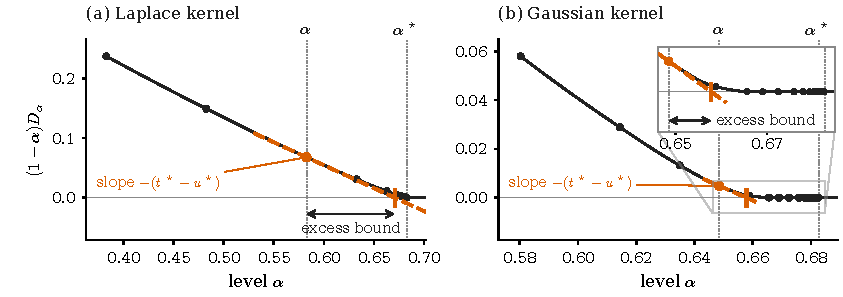
\includegraphics[width=\textwidth]{figs_aos/fig_excess_aos.pdf}
\caption{The rescaled path $(1-\alpha)D_\alpha$ for $P=N(1,1)$ and $Q=N(-1,1)$, whose total variation is
$\alpha^\star=2\Phi(1)-1\approx\fxAlphaStar$, with the Laplace kernel (a) and the Gaussian kernel (b), both with
$\sigma=1$ (dots: computed levels; line: monotone interpolation). At $\alpha=\fxLevelLap$ in (a) and
$\alpha=\fxLevelGauss$ in (b) the dashed line of slope $-(t^\star-u^\star)$ supports the path; the excess of the
population ramp over $\alpha$ is at least the distance (arrow) from $\alpha$ to the zero of the line (tick), by
Proposition~\ref{prop:excess}, and the inset of (b) enlarges the region near $\alpha^\star$. That distance is a fraction
$\fxFracLap$ of $\alpha^\star-\alpha$ for the Laplace kernel and $\fxFracGauss$ for the Gaussian kernel at this level,
closer to $\alpha^\star$. The Gaussian fraction, $\fxFracGaussAtLap$ at $\alpha=\fxLevelGaussAtLap$, falls toward zero
as $\alpha\uparrow\alpha^\star$, where its path is flatter than every power.}
\label{fig:excess}
\end{figure}

\subsection{Touching contaminations, and why the margin is pessimistic}
\label{sec:touching}

Under the hypotheses of Proposition~\ref{prop:newsobolev}, Theorem~\ref{thm:loratemain} guarantees at least the rate
$(n\wedge m)^{-2/(2s+3)}$, $(n\wedge m)^{-2/5}$ for the Laplace kernel, which Theorem~\ref{thm:laplacerate} improves to
$(n\wedge m)^{-1/2}$, up to powers of $\log(n\vee m)$, under one more condition, for samples of comparable size. Under those of Proposition~\ref{prop:newgauss} the margin
guarantees at least the logarithmic rate $c/\log(n\wedge m)$ for every $c>\pi^2\sigma^2\ell_0/4$, on grids with at
most $(n\wedge m)^b$ levels for a fixed $b$ (Proposition~\ref{prop:newrates} of the supplement), in both cases up to the
mesh. For the split-sample bound we prove no converse. For the analytic baseline run with the larger threshold
$\tau^{\mathrm S}$ the margin rate cannot be improved for Sobolev kernels, and with the Gaussian kernel its error is
not $O((n\wedge m)^{-a})$ for any $a>0$ (Proposition~\ref{prop:newconverse} of the supplement); for
$\tau^{\mathrm P}$ no converse is known.

The margin is pessimistic. Theorem~\ref{thm:loratemain} bounds the excess $\E_P\rp-\E_Q\rp-\alpha$ of the population
ramp from below by $D_\alpha/(\beta\Delta_\phi)$ (Lemma~\ref{lem:popramp} of the supplement), replacing the gap
$t^\star-u^\star$ between its cut points by its largest value $\Delta_\phi$. The gap is a slope of the rescaled
path $(1-\alpha)D_\alpha$, the distance between the parts of mass $1-\alpha$ that the trimmings keep, which is convex in
$\alpha$ (Lemma~\ref{lem:pathconvex} of the supplement). The line through the point of the rescaled path at $\alpha$
with slope $-(t^\star-u^\star)$ supports it, and the excess of the ramp is at least the distance from $\alpha$ to the
zero of this line (Proposition~\ref{prop:excess}, Figure~\ref{fig:excess}). When the path lies between two multiples of one power of
$\alpha^\star-\alpha$, this distance is a fixed fraction of $\alpha^\star-\alpha$.

\begin{proposition}[Excess of the population ramp]
\label{prop:excess}
Let Assumption~\ref{ass:regularity} hold, let $0<\alpha^\star<1$, let $\alpha<\alpha^\star$, let $f^\star$ be the
direction of the population witness, $t^\star$ the smallest $(1-\alpha)$-quantile of $f^\star(X)$ and $u^\star$ the
largest $\alpha$-quantile of $f^\star(Y)$, so that $t^\star-u^\star\ge D_\alpha>0$ (Lemma~\ref{lem:popramp} of the
supplement), and let $\rp^\star$ be the ramp of $f^\star$ between $u^\star$ and $t^\star$. Then:
\begin{enumerate}[label=(\roman*),leftmargin=*]
\item $\E_P\rp^\star-\E_Q\rp^\star-\alpha\ge(1-\alpha)D_\alpha/(t^\star-u^\star)$, and
$(1-\alpha')D_{\alpha'}\ge(1-\alpha)D_\alpha-(t^\star-u^\star)(\alpha'-\alpha)$ for every $\alpha'\in[0,1)$;
\item if $c_1\epsilon^\gamma\le D_{\alpha^\star-\epsilon}\le c_2\epsilon^\gamma$ for $0<\epsilon\le\epsilon_0\le\alpha^\star$, then
at $\alpha=\alpha^\star-\epsilon$ with $\epsilon\le\epsilon_0/2$ the excess in (i) is at least
$(1-\alpha^\star)c_1\epsilon/(2^\gamma c_2)$, and this holds under the hypotheses of Proposition~\ref{prop:newsobolev};
\item for the Laplace kernel $e^{-|x-y|/\sigma}$ on $\R$, $u^\star\le f^\star\le t^\star$ on $\R$ and the first
inequality of (i) is an equality.
\end{enumerate}
\end{proposition}

On the line, by part (iii), the Laplace witness is already clipped at its cut points, and so is the witness fitted on
the data, whose ramp maximizes the ratio of empirical excess to RKHS norm over functions of oscillation at most one
(Lemma~\ref{lem:lapclip} of the supplement). Comparing this ratio with the population path at two levels shows that the
fitted ramp keeps a fixed fraction of the excess of the population ramp (Proposition~\ref{prop:lapfitted}).

\begin{theorem}[Near-parametric rate with the Laplace kernel]
\label{thm:laplacerate}
Let $P,Q$ satisfy the hypotheses of Proposition~\ref{prop:newsobolev} on the laws, let $n\wedge m\ge10$, and compute
$\widehat\alpha$ as in Theorem~\ref{thm:loratemain}, on a grid of $J$ levels in $(0,1)$ with mesh $\Delta_{\mathcal G}$
below $\alpha^\star$, with the kernel $e^{-|x-y|/\sigma}$, $\sigma>0$ fixed in advance, an exact minimizer of
\eqref{eq:qp} at each level, and, in place of the one-rank tolerance \eqref{eq:cutrank}, cut points that are genuine
empirical quantiles of the witness values, computed with or without each point's own term in \eqref{eq:witness}. Let
$\eta\in(0,1)$, $L_\delta=\log(1/\delta)$, $L_{n,m}=\log\{(n\vee m)/\eta\}$ and
$B_{n,m}=v_{\min}^{-2}\{L_\delta^{1/2}+(\log(2J/\eta))^{1/2}\}(n\wedge m)^{-1/2}$.
\begin{enumerate}[label=(\roman*),leftmargin=*]
\item If for some $r_\ast\in(0,1]$ and $c_\ast>0$
\begin{equation}
|p(x)-q(x)|\ \ge\ c_\ast\min(r_\ast,|x-x_0|)\,\{p(x)+q(x)\}\qquad\text{for almost every }x,
\label{eq:condR}
\end{equation}
then with probability at least $1-\delta-\eta$,
\[
\alpha^\star-\Delta_{\mathcal G}-O\big(L_{n,m}^{3/4}(n\wedge m)^{-1/2}+B_{n,m}\big)\ \le\ \widehat\alpha\
\le\ \alpha^\star .
\]
\item If instead $(P+Q)(\{x:|x-x_0|>t\})\le C'e^{-t/C'}$ for all $t>0$, the same holds with
$L_{n,m}^{2/3}(n\wedge m)^{-4/9}$ in place of $L_{n,m}^{3/4}(n\wedge m)^{-1/2}$.
\end{enumerate}
The constant in the $O$ depends only on $\sigma$ and on the pair, as stated in Theorem~\ref{thm:laplaceconst} of the
supplement.
\end{theorem}

Under these hypotheses $\TV(P,Q)=F_Q(x_0)-F_P(x_0)$ is a one-sided Kolmogorov distance, which the one-sided
Kolmogorov--Smirnov statistic bounds from below at the rate $(n\wedge m)^{-1/2}$, with no condition on the likelihood
ratio and no logarithmic factor. The interest of the theorem is that a kernel bound that does not sort the
data, and returns the set, attains this rate up to logarithmic factors, which the margin does not see; it is no reason
to prefer the method on the line. Condition \eqref{eq:condR} asks that $p/q$ stay away from one off every neighborhood of $x_0$, so it excludes
contaminations local to a common core, with $p=q>0$ on an interval, where only part (ii) applies. No multivariate theorem
singles out the Laplace kernel in $\R^d$, where its choice rests on this one-dimensional theory and on its power against
differences of high frequency, seen on a one-dimensional oscillating density (Section~\ref{sec:numharder}). Section~\ref{sec:laplaceproof} of the supplement discusses
the exact minimizers the theorem needs, its constants, whose uniformity over a class is open, and a simulation.
